\chapter{Scientific Background}
\label{cha:chapter2}

A time series is a set of data points with a clear ordering in time. Some examples are the exchange rate between two currencies over time or the electricity consumption of households, see Figures \ref{fig:example_timeseries} and \ref{fig:example_timeseries_electricity} \cite{gluonts_paper}.

\begin{figure}[htb]
  \centering
  \minipage{0.47\textwidth}
  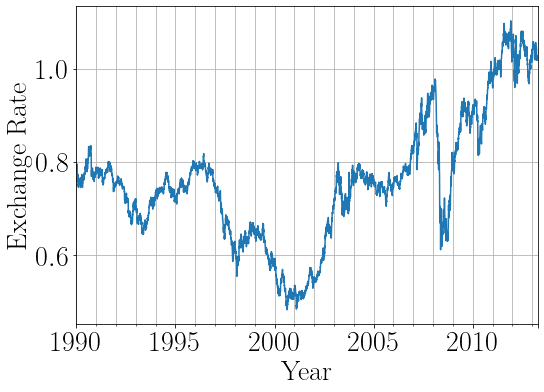
\includegraphics[width=\linewidth]{./img/exchange_rate_zoomed_2.png}
  \caption{Exchange rate of two currencies from 1990 to 2013.}
  \label{fig:example_timeseries}
  \endminipage\hfill
  \minipage{0.47\textwidth}
  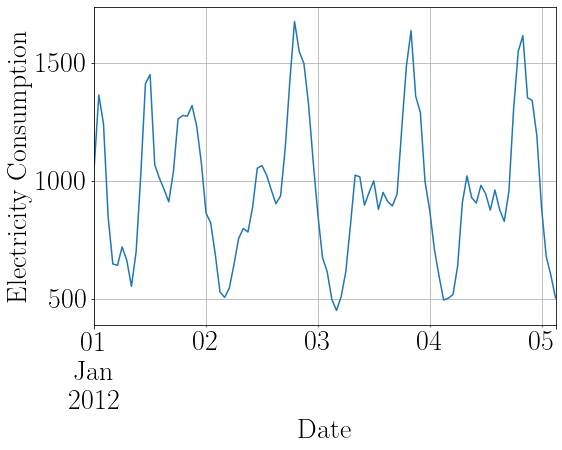
\includegraphics[width=\linewidth]{./img/electricity_zoomed_3.png}
  \caption{Household electricity consumption.}
  \label{fig:example_timeseries_electricity}
  \endminipage\hfill
\end{figure}

Timeseries which increase or decrease in value over a longer period of time is said to have a upward or downward \textit{trend}. If a timeseries has evenly distributed patterns such as the spikes in Figure \ref{fig:example_timeseries_electricity} the timeseries is said have a seasonal component with a frequency equal to the distance between the spikes. For the electricity timeseries this would be 24 as household electricity consumption follow the daily rythm of everyday life i.e. use more energy during the morning and evening with 24 hour intervals. If the timeseries exhibit spikes without a clear frequency, these are knowns as \textit{cycles} \cite{bauer2021libra}. The data which cannot be described by these features is known as the \textit{remainder} \cite{hyndman_forecasting_3rd}. Not all timeseries exhibit all of these patterns, for example, the timeseries in Figure \ref{fig:example_timeseries_electricity} does not display a trend.

\section{Time Series Decomposition}
Timeseries decomposition is the act of extracting features such as the seasonality and trend from timeseries data. This is often done in order to gain understanding of the data \cite{hyndman_forecasting_3rd}. While several methods of performing time series decomposition exists, one of the most powerful methods commonly used is STL decomposition \cite{hyndman_forecasting_3rd}. After a timeseries has been split into its constituents one can quantify the strength of the trend and seasonality apparent in the data. This is done through compairing the variances of the seasonality \(S\) and trend \(T\) with that of the residual \(R\). The strength of the trend \(F_t\) is then calculated according to Equation \ref{eq:strength_of_trend} and the strength of the seasonality \(F_s\) is calculated according to Equation \ref{eq:strength_of_seasonality}.

\begin{figure}[h]
  \[ F_t = max(0,1-\frac{Var(R)}{Var(T + R)}) \]
  \caption{Equation for calculating the strength of the trend of a timeseries.}
  \label{eq:strength_of_trend}
\end{figure}

\begin{figure}[h]
  \[ F_s = max(0,1-\frac{Var(R)}{Var(S + R)}) \]
  \caption{Equation for calculating the strength of the seasonality of a timeseries.}
  \label{eq:strength_of_seasonality}
\end{figure}

\section{Time Series Forecasting}
\label{sec_time_series_forecasting}
Time series forecasting is the art of predicting future trends of time series based on past observations. It is a key technology within many fields and is fundamental to the business decision process for many companies. Being able to interpret timeseries in order to predict future trends makes it possible to plan for the future. For example power generation companies can adjust the amount of electricity which should be generated to match the expected demand and banks could make informed decisions about possible investment opportunities. There are many methods of generating such predictions, ranging from the use of simple heuristics to complex machine learning methods \cite{hyndman_forecasting_3rd}. An overview of how to use deep learning to generate such forecasts is presented in Section \ref{sec:deep_learning_methods} and several state of the art forecasting models are presented in Section \ref{algorithms}.

Time series forecasting differs from common machine learning tasks such as image recognition or language processing in that predictions are not binary. More specifically, in time series forecasting a prediction is expected to be a close estimate of future values. Thus, quantifying the magnitude of the error from the ground truth is of importance in order to properly evaluate the accuracy of a forecasting model. This is commonly done by calculating an error metric, the choice of which varies depending on what is being forecasted and on preference of the forecasting practitioner. \cite{hyndman_forecasting_3rd,hyndman_measuring_nodate, willmott_advantages_2005} In Section \ref{subsec:error_metrics} some such error metrics are presented.

Forecasts often comes in one of two forms; probabilistic forecasts or point forecasts. A point forecast is a forecast which consist of only one estimation of future values. This estimation could be either a single point in time or a series of points for several different timesteps. In Figure \ref{fig:example_timeseries_forecast_point} an example of a point forecast for several timesteps can be seen. Point forecasts has the disadvantage that they do not confer how accurate they are which may lead to prectitioners being overly confident in the forecasts. This has historically caused several issues and more recently with covid-19 where over relying on point forecasts led to overly drastic measures for governments and hospitals \cite{IOANNIDIS2020}. Probabilistic forecasts such as the one in Figure \ref{fig:example_timeseries_forecast_probabilistic} includes this information by generating prediction intervals of the forecasts.

\begin{figure}[htb]
  \centering
  \minipage{0.5\textwidth}
  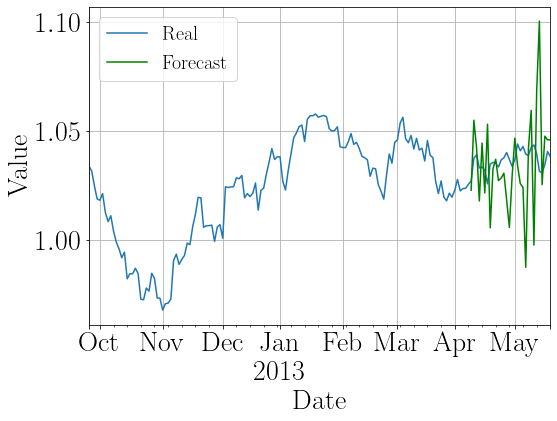
\includegraphics[width=\linewidth]{./img/exchange_rate_point_forcast.png}
  \caption{Point forecast}
  \label{fig:example_timeseries_forecast_point}
  \endminipage\hfill
  \minipage{0.5\textwidth}
  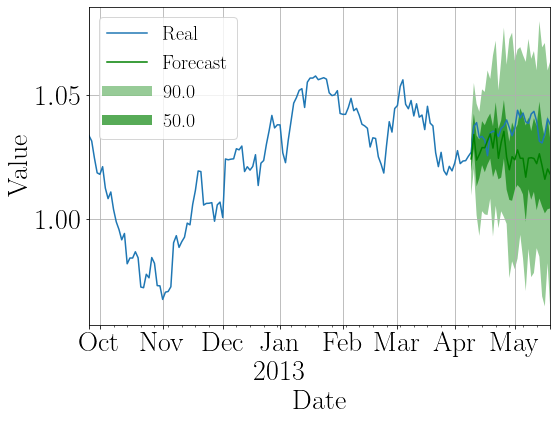
\includegraphics[width=\linewidth]{./img/exchange_rate_prob_forcast.png}
  \caption{Probability forecast}
  \label{fig:example_timeseries_forecast_probabilistic}
  \endminipage\hfill
\end{figure}

Many methods exist for generating forecasts on timeseries data, two common groups of these are machine learning based methods and trivial methods. A trivial forecasting method would be, for example, to predict that the next value should be the same as the last recently observed value or the average of the last N observations. For certain timeseries, trivial methods perform competitively and as such these are often held as a baseline to which new forecasting methods are being compared too. Some more complex methods include those based on regression analysis such as linear regression or autoregressive models such as ARIMA \cite{hyndman_forecasting_3rd}. Autoregressive models are a subset of regression models where the temporal ordering of the datapoints matter. I.e. autoregressive models use past observations to predict future values.

Lately, inspired by the successful use of neural networks in other domains, several neural network based approaches for time series forecasting have been introduced. Early implementations such as simple multi-layered perceptrons did not perform competitively with the more classical approaches such ARIMA. However modern deep learning models such as DeepAR \cite{salinas_deepar_2019} and MQCNN \cite{wen_multi-horizon_2018} have reported highly competitive accuracies.

Forecasting models for forecasting can also be split into further sub families such as whether they are local or global models. Local models are trained on individual time series while global models are trained on all time series in the training set. Essentially for a dataset with N timeseries, if using local models, one will have N individually trained models. If the algorithm would be a global model then only a single model would be used for all N timeseries in the dataset. Generally speaking, local models performs well for timeseries with much historical data. However for short or new timeseries, local models often perform poorly due to the inability to train the model on sufficiently large amounts of data points. This is known as the cold start problem. Since global models train on the entire dataset across all timeseries, the length of any individual timeseries has less of an impact. I.e. generally global models suffer less from the cold start issue as the global model can use data from other timeseries as a basis for its predictions \cite{wang_deep_2019}.

So far, we have seen the time series forecasting problem as generating a forecast from a single timeseries for example predicting future temperatures based on previously recorded temperatures. Predicting using singular timeseries such as this is known as univariate forecasting. Another family of forecasting solutions leverage related timeseries when making predictions. For example temperatures may depend on cloud coverage or the hours of sunlight. Algorithm which leverage information from related timseries are known as multivariate algorithms. The benefits of multivariate forecasting is that trends or patterns can be identified using these related timeseries in order to improve the accuracy for the target variable. For example, the temperature is higher whenever there is a large amou8nt of sun hours and no clouds.

\section{Evaluating Forecasting Performance}
\label{sec:evaluating_performance}
If a model generates forecasts it is important to be able to quantify how good or bad its predictions are. This is generally done via a process called backtesting. When backtesting, first the algorithm is trained on a dataset, thereafter, the trained algorithm generates predictions on a test dataset. The generated predictions from the algorithm are then compared to the ground truth and a suitable error metric quantifying how wrong the prediction was from the expected value is calculated.

In other machine learning domains such as image recognition, the datasets used for training the models are disjoint from the test datasets. However, in the domain of time series forecasting this is not the case. Generally the train set contains the same time series as in the test set except for the last couple of data points for each time series. The number of removed data points is commonly the number of timesteps that a model should predict \cite{hyndman_forecasting_3rd}. In Figure \ref{fig:train_test_split} a train test split is presented of a time series with six data points. In this example, a forecasting algorithm should predict one timesteps into the future, thus, the last datapoint would be removed and the train set would contain five data points while the test series would contain six.

\begin{figure}[htb]
  \centering
  \minipage{1\textwidth}
  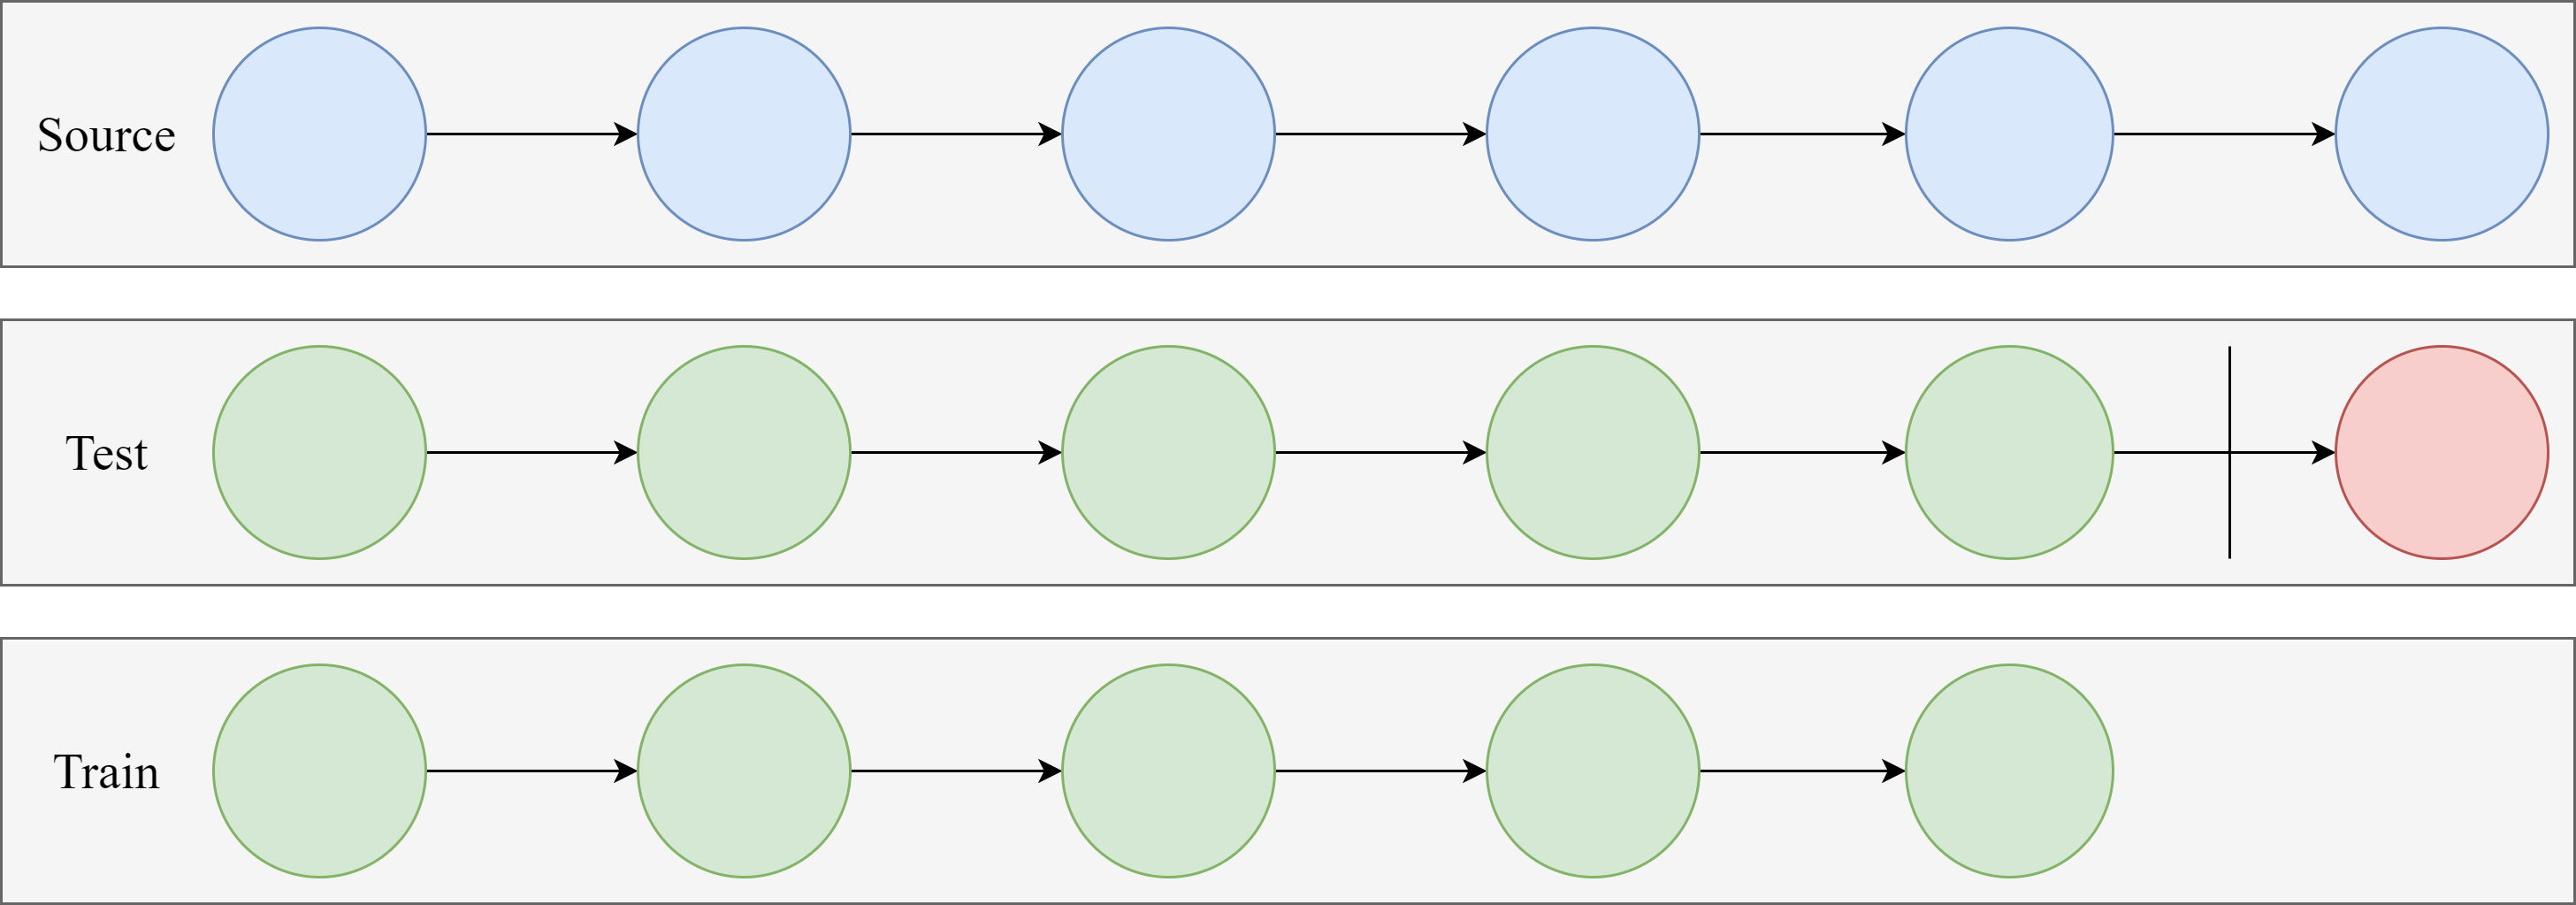
\includegraphics[width=\linewidth]{./img/train_test_split.png}
  \caption{An example train test split of a time series with six datapoints. The red circle is the datapoint which prediction will be compared to.}
  \label{fig:train_test_split}
  \endminipage\hfill
\end{figure}


A popular method of increasing the amount of test data is to make the test dataset contain multiple copies of each time series where each one is successively shorter. The train dataset would contain the shortest of the truncated time series truncated one additional time. This process is called K-fold cross validation but is also known as forecasting on a rolling origin or time series cross validation. Performing a 3-fold cross validation on a dataset containing one time series of length six timesteps would result in a dataset containing three time series. An example of this is shown in Figure \ref{fig:k_fold_validation}. The advantage of the larger test dataset generated by this approach is that the performance of a model can be more accurately determined as it is excercised on more unseen data \cite{hyndman_forecasting_3rd}.

\begin{figure}[htb]
  \centering
  \minipage{1\textwidth}
  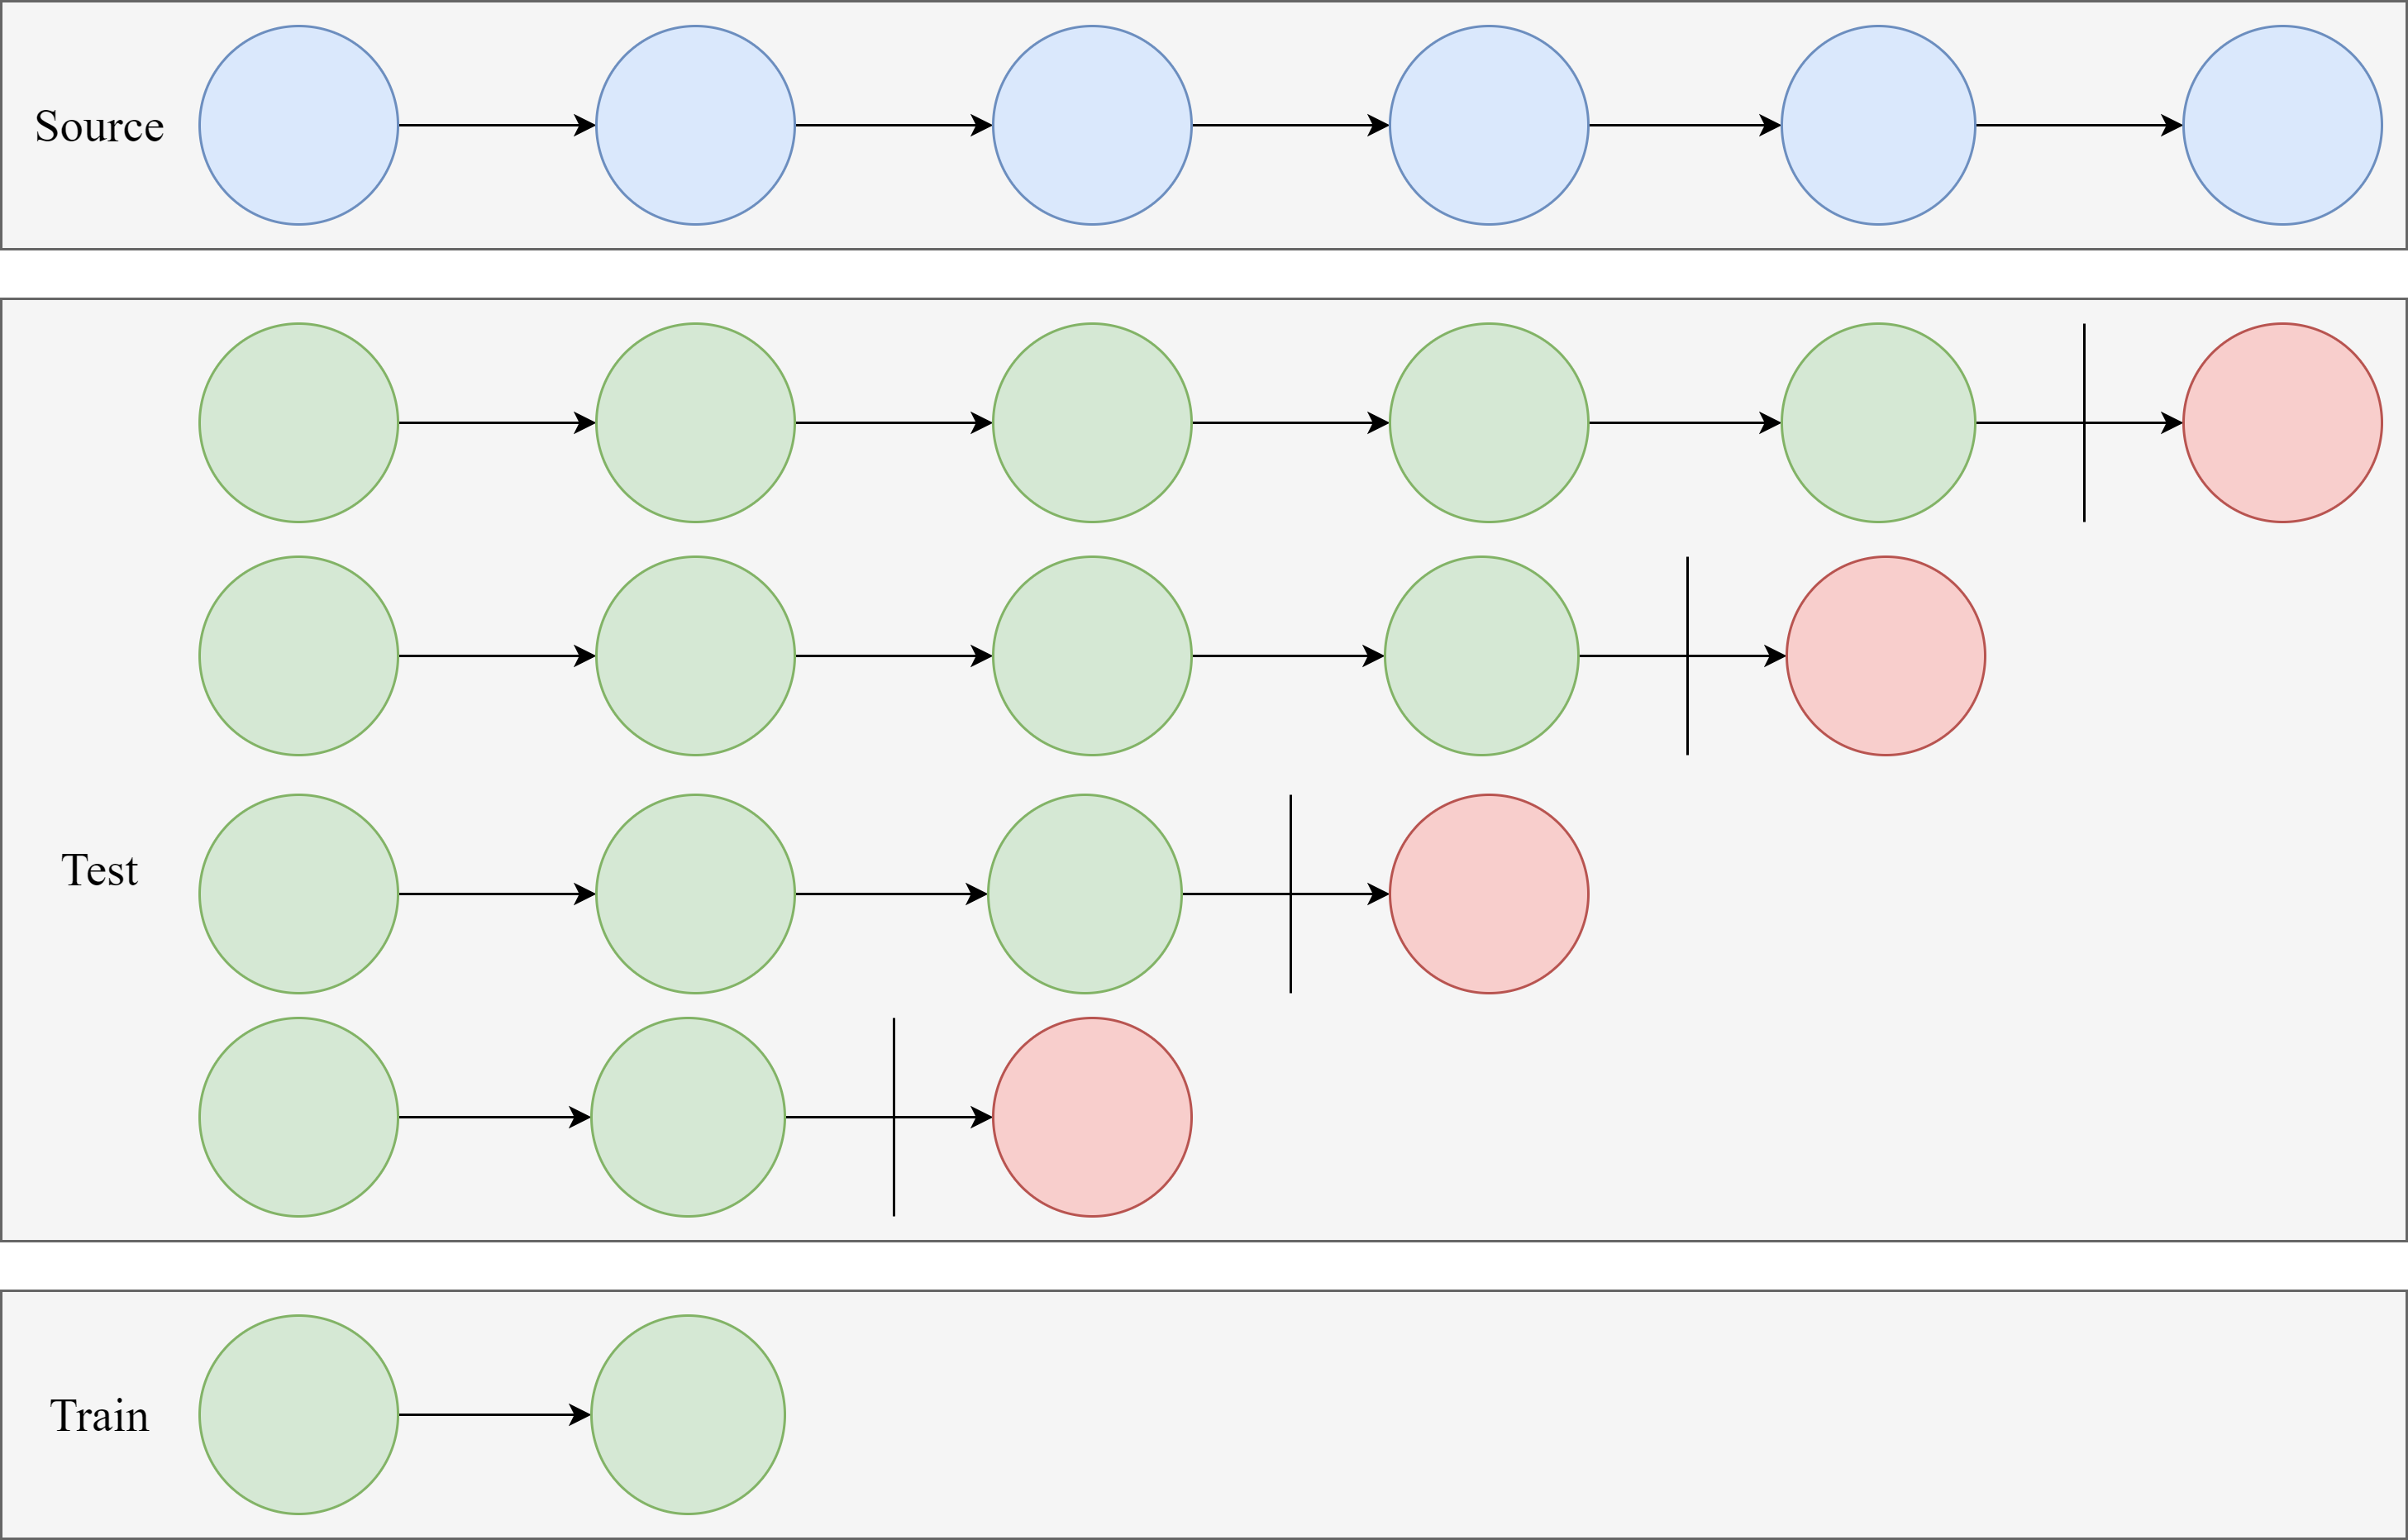
\includegraphics[width=\linewidth]{./img/k_fold_validation.png}
  \caption{Example of a four fold cross validation dataset split. The red circles are the datapoints which predictions will be compaired to. Worth noting is that the train dataset here only has one timeseries of length two, i.e. one less than the shortest timeseries in the test dataset. This example assumes a prediction length for the dataset of one datapoint.}
  \label{fig:k_fold_validation}
  \endminipage\hfill
\end{figure}


\subsection{Error Metrics}
\label{subsec:error_metrics}
When a forecasting model generates predictions on a timeseries, one needs to be able to quantify the error of the prediction from true observed values. In order to do this many different error metrics exists each with its own benefits and drawbacks. Often the choice of metric is dependent on data, and business application where the prediction will be used. In this section some of the error metrics which are commonly occurring in literature are presented. These metrics are calculated automatically when performing a backtest in Gluon-TS, see \ref{subsec:gluonts_overview} for details about this process. Note that only a subset of the metrics available in Gluon-TS is presented here to form a basis for subsequent chapters.

Error metrics for forecasting can generally be split into three different categories: scale-dependent, scaled and percentage based \cite{hyndman_forecasting_3rd}. Within each of these categories multiple different metrics exists. The remainder of this section describes some common error metrics within each category along with pros and cons and how they are calculated. For the rest of the thesis, a forecast is referred to as \(\hat{Y}\) and the expected values are referred to as \(Y\).

\subsubsection{Absolute Error}
The absolute error is calculated as the distance between the predicted value and the ground truth. An absolute error is positive and a value of 0 is optimal. It is an intuitively simple error, thus it can easily be understood and discussed when comparing algorithms.

However intuitive the absolute error is, there is a a key issue with this error and that is that it is scale dependent. I.e. the greater the values of the dataset being predicted on, the larger the absolute error will be. This makes it impossible to compare the accuracy of an algorithm across different datasets unless they have the same scale. \cite{hyndman_forecasting_3rd} Furthermore, scale dependent metrics such as these may not be suitable even for comparing between timeseries within a single dataset. Imagine a dataset such as the electricity dataset (see Table \ref{tab:datasets}) where each timeseries is the electricity consumption from a household. One household may contain many people and appliances while another may be a factory full of equipment with high power demands. These two timeseries would have two very different scales thus making it hard to compare the accuracy of the predictions.

\begin{figure}[h]
  \[Absolute Error = \sum|Y - \hat{Y}|\]
  \caption{Equation for calculating the absolute error}
  \label{eq:abs_error}
\end{figure}

\subsubsection{Root Mean Squared Error - RMSE}
\label{sec:RMSE}
The root mean squared error is another scale dependent error such as the absolute error. RMSE is calculated by taking the square root of the mean of the squared error. The RMSE thus punishes larger errors more than smaller errors. The RMSE is more complicated to interpret than for example the Absolute Error due to the non-linear nature, despite this, RMSE is widely used in practise \cite{hyndman_forecasting_3rd,gluonts-github}.

\begin{figure}[h]
  \[RMSE = \sqrt{mean((Y - \hat{Y})^2)}\]
  \caption{Equation for calculating RMSE}
  \label{eq:RMSE}
\end{figure}

\subsubsection{Mean Absolute Percentage Error - MAPE}
Percentage based errors such as the Mean Average Percentage Error normalizes the errors between 0 and 1 thus MAPE can be compared across datasets with different scales. While this is beneficial, MAPE suffer from other issues. For example MAPE becomes infinite or undefined if the ground truth is 0 for any parts of the prediction. Further issues exists for example that it penalizes negative errors more than positive errors. These issues has lead to variations of MAPE to be created such as Symmetric MAPE \cite{hyndman_forecasting_3rd,gluonts-github}.

\begin{figure}[h]
  \[MAPE = mean(\frac{|Y - \hat{Y}|}{|Y|}))\]
  \caption{Equation for calculating MAPE}
  \label{eq:MAPE}
\end{figure}

\subsubsection{Mean Absolute Scaled Error - MASE}
MASE is a metric which takes the average error across all timeseries and scale is based on the error from a reference forecasting. An example a model which MASE uses for reference would be the Naive2Estimator detailed in Section \ref{model:naive2}. Scaling the forecasting error in this way causes the MASE metric to be scale independent which makes it suitable when comparing across datasets. A MASE of 1 corresponds to that the algorithm under test is equally good as the naive model. A MASE below 1 means that the current model performs better than the naive model while a MASE above 1 means that the model performs worse than the naive baseline model \cite{hyndman_forecasting_3rd,gluonts-github}.

In certain scenarios, for example if the reference model would result in a perfect prediction a division by zero would occur and MASE would tend towards infinity. This is a major drawback of the MASE metric which renders it unusable for certain datasets.

In equation \ref{eq:MASE} the denominator is the mean error of a seasonal naive model. \(Y_t\) means the value at time \(t\) and \(Y_{t-m}\) means the value of the timeseries at the previous period, i.e. if the expected seasonality is 24h \(Y_{t-m}\) would become the value 24 timesteps previously.

\begin{figure}[h]
  \[MASE = \frac{mean(|Y - \hat{Y}|)}{mean(|Y_t - Y_{t-m}]|)}\]
  \caption{Equation for calculating MASE}
  \label{eq:MASE}
\end{figure}

\subsubsection{Mean Scaled Interval Score - MSIS}
\label{sec:msis}
Since probabilistic forecasts do not generate point predictions but prediction intervals these can also be scored in regards to how often these contain the true values \(Y\). The MSIS metric penalizes wide prediction intervals in two ways. First, the absolute width of the prediction intervals is penalized. Secondly, the distance from the edge of the prediction interval from the expected value \(Y\) is penalized. Thus smaller more accurate and consistent prediction intervals are encouraged \cite{makridakis_m4_2020}. In Equation \ref{eq:MSIS} \(\hat{Y_u}\) is the upper limit of the forecast prediction interval and \(\hat{Y_l}\) is the lower boundrary. The \(\alpha\) parameter is the significance level used, this is commonly set to 0.05 to evaluate the 95\% prediction intervals \cite{makridakis_m4_2020,gluonts-github}. The \(I(x)\) function is the indicator function which is 1 if \(\hat{Y}\) is within the prediction interval and 0 otherwise. The denominator used in Equation \ref{eq:MSIS} is the mean seasonal error, i.e. the same denominator for the MASE metric. This division makes the MSIS metric scale independent \cite{gluonts-github,makridakis_m4_2020}.

\begin{figure}[h]
  \[msis = \frac{mean(\hat{Y_u} - \hat{Y_l} + \frac{2(\hat{Y_l}-Y)}{\alpha}I(Y<\hat{Y_l}) + \frac{2(Y-\hat{Y_u})}{\alpha}I(Y>\hat{Y_u}))}{mean(|Y_t - Y_{t-m}]|))}\]
  \caption{Equation for calculating MSIS}
  \label{eq:MSIS}
\end{figure}

\section{Deep Learning Forecasting Methods}
\label{sec:deep_learning_methods}
Neural Networks (NN) have in recent years been successfully applied in many different domains such as image recognition and natural language processing. However, within the field of forecasting NN based approaches has performed subpar compared to more traditional statistical methods \cite{m3_competition,makridakis_m4_2020,oreshkin_n_beats_2020, other_thesis}. This relative inefficiency between NN based approaches and classical methods and the success of NN in other domains has resulted in much research being made in improving tools and NN based models for forecasting \cite{gluonts_paper}.

A simple neural network, similar in architecture to the network described in Section \ref{algo:simplefeedforward} is presented in Figure \ref{fig:simplefeedforward}.

\begin{figure}[htb]
  \centering
  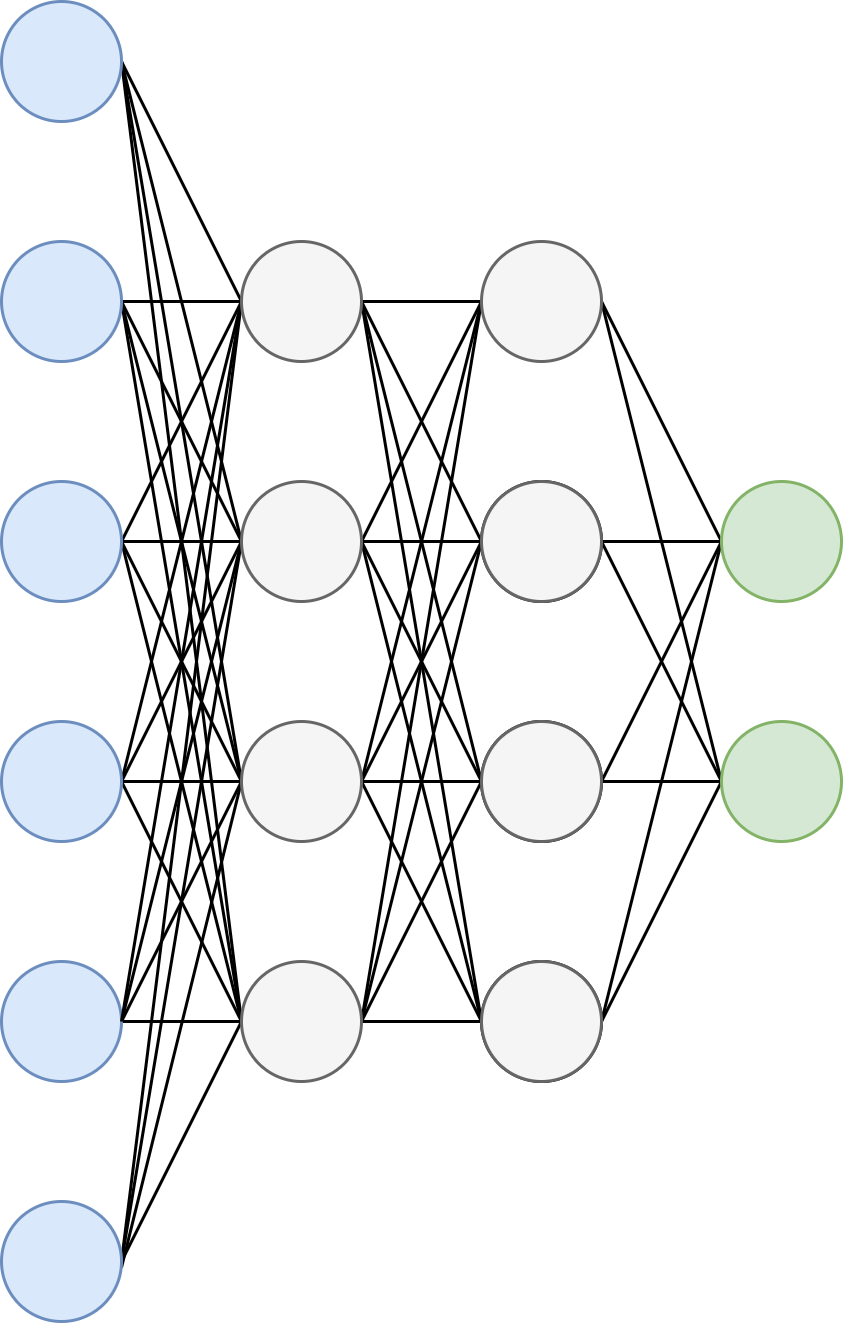
\includegraphics[width=0.5\linewidth]{./img/simplefeedforward.png}
  \caption{A simple neural network for forecasting based on the SimpleFeedForwardEstimator in Section \ref{algo:simplefeedforward}.}
  \label{fig:simplefeedforward}
\end{figure}
\clearpage

This very small network consists of four fully connected layers of different sizes with six input nodes, two fully connected hidden layers with four nodes each, and an output layer of two nodes. In this network, the input layer (marked in blue) has the same amount of nodes as the number of timepoints in the past which the network should make use of. This is will in the remainder of the thesis be called the \textit{context length} of the network. The output nodes (in green) for this network produce a prediction of two timesteps. Thus this network has a \textit{prediction length} of two timesteps. The context length and the desired prediction length are often exposed as hyperparameters for time series forecasting algorithms since they vary between datasets.

An issue with the simple network in Figure \ref{fig:simplefeedforward} is that each timestep in the forecast is not influenced by the previous one. i.e. the prediction at timestep \(N\) does not depend on the prediction at timestep \(N-1\). In real life scenarios, timeseries data often has a temporal dependency, for example, the temperature two days from now is affected by the temperature of tomorrow. This dependency is lost in simple neural network architectures such as this one. An alternative neural network architecture which can make use of temporal effects is known as a Recurrent Neural Network (RNN).

RNNs reuse the output of their nodes as inputs for the next iteration of the algorithm. This recurrent link causes previously seen values in the sequence to be represented in a hidden internal state. While this makes RNNs suited for use with sequential data such as time series, they become hard to train successfully as long term dependencies are lost \cite{bengio1994learning}. One of the most successful techniques for use in RNNs to solve this is the Long Short-Term Memory (LSTM) node architecture. LSTM nodes enables RNNs to remember previously seen data for longer and forget or ignore parts of it \cite{sherstinsky_fundamentals_2020}.

Some issues with NN based approaches is that they require a large amount of data to be trained on properly. This is due to the fact that NNs are prone to overfit which makes them unable to generalize well to new data \cite{srivastava_dropout_2014}. Despite this, NN has several advantages over classical approaches such as the capability to learn non-linear patterns from the data. Additionally, NN models are capable of cross learning between related time series without the need of manual feature extraction \cite{smyl_hybrid_2020}.

\subsection{Sources of Randomness}
\label{subsec:sources_randomness}
Neural networks heavily rely on random processess to function and thus randomnes is introduced at several points in a forecasting workflow. Some randomness can be introduced whenever an neural network is initialized as the weights and biases of a networks often are set randomly. Similarly, when training a neural network randomness can be introduced if optimization techniques such as dropout is used as dropout randomly sets weights in the network to 0 at certain points in the training loop which causes the algorithm to be less prone of overfitting the data \cite{srivastava_dropout_2014}. Even the method used for training neural networks, stochastic gradient descent introduces randomness.

Deep NNs are notoriously slow to train when compared to many other methods, thus lowering the time spent for training and inference is often done by parallelizing algorithms such that they run on several threads on a CPU or on hardware accelerators such as GPUs, FPGAs or ASICs. The execution speed of a forecasting model is thus highly dependent on what hardware the models are running on, however the hardware configuration also impacts the variance of the accuracy of ML models \cite{zhuang2021randomness}. Parallelization of an algorithm often introduces a larger amount of data shuffling which impacts the rate of convergence of an algorithm. Parallelizing a forecasting model may make it unstable so that it cannot converge as will be shown in chapter \ref{cha:chapter6}. Due to this it is important that the hardware used when training and tuning forecasting models is presented in detail so that results can be properly reproduced \cite{pineau2020improving}.

A common method for reducing the randomness associated with ML models is to fix the seed used by the random number generator to a known number. While this removes randomness from for example random initializations or from backpropagation \cite{beam2020challenges}, other sources of randomness such as that introduced by the hardware or the OS remain. Furthermore, fixing the seed can be seen as an additional hyperparameter which needs to be tuned as it directly impacts the predictive performance of forecasting methods. While there are some major benefits of fixing the seed, there are also drawbacks. For example,luck becomes a factor in what accuracy can be expected for an algorithm. I.e. the accuracy of a model may seem highly competitive while if another seed would be used the accuracy of the model could change significantly \cite{beam2020challenges}. In real life usecases such as when forecasting are used in companies or organizations, setting the seed may be beneficial or even necessary in order to optimize its performance for an individual task. In research however, setting the seed without reporting what it was can bias results and make them technically irreproducible \cite{beam2020challenges,pineau2020improving,bouthillier2021accounting}.

One method of lowering the variance of machine learning methods is to use ensambles of forecasting methods as per the Bootstrap AGGregatING (Bagging) technique \cite{buhlmann2002analyzing}. An ensamble is a set of multiple different ML models with slightly different configurations which are all trained in parallel.Bagging extends this such that a the input dataset is randomly sampled to create multiple independent datasets. Each model is then trained on one of these datasets and their forecasts are then combined via some voting or weighting scheme \cite{buhlmann2002analyzing}. While bagging is often associated with decision trees they are also suitable for use with deep learning forecasting models such as the N-BEATS Ensamble Estimator discussed in Section \ref{algo:nbeats}.

K-fold cross validation which was discussed in Section \ref{sec:evaluating_performance} can also lower the variance of forecasting algorithms as it introduces multiple different train-test splits from a single dataset \cite{buhlmann2002analyzing}.

\section{Benchmarking}
\label{sec:related_work}

Backtesting is a fundamental part of benchmarking, however benchmarking is also concerned with ensuring that different models can be fairly and reproducibly compared to each other \cite{huang_benchmarking_2019}. In other domains of machine learning several benchmarking solutions exists, most notably MLPerf \cite{mattson_mlperf_2020}, MLBench \cite{noauthor_mlbench_nodate}, DLBS \cite{vassilieva_deep_nodate} and UCR \cite{dau2019ucr}. Despite the success of benchmarks in other ML domains no established “go-to” benchmark exists in the domain of time series forecasting \cite{huang_benchmarking_2019}.

Attempts has been made to create such a benchmark, one such example is \textit{Libra} \cite{bauer2021libra} which uses custom datasets containing timeseries sampled from various well known datasets. The sampling methodology used in Libra was aimed to create datasets with a high amount of diversity between the timeseries. Due to this diversity, the datasets in Libra are not suitable for global forecasting models as they are highly unrelated. In a nutshell, Libra focuses on benchmarking the accuracy and time-to-result for univariate forecasts generated by local models.


\begin{table}[h]
  \begin{tabularx}{\textwidth}{|l|c|c|c|c|X|}
    \hline
    Name    & TS & Integration    & DS & Focus & Info                                                                    \\
    \hline
    \hline
    Libra   & X  & R              & X  & A, S  & Diverse datasets for univariate local models                            \\
    \hline
    UCR     & X  & CSV            & X  & A     & Dataset repository with reference accuracies.                           \\
    \hline
    MLPerf  &    & Docker, CLI    &    & S     & Benchmarking for hardware and ML frameworks                             \\
    \hline
    PMLB    & X  & Python, R      & X  & -     & Dataset repository with 298 datasets for regression and classification. \\
    \hline
    MLBench &    & Kubernetes     &    & S     & For distributed ML frameworks                                           \\
    \hline
    DLBS    &    & Docker, Python &    & S     & Benchmarking for hardware and ML frameworks                             \\
    \hline
  \end{tabularx}
  \caption{Overview of six benchmarking suites for ML, the column marked TS depicts whether they support time series forecasting and the DS column is whether they offer custom datasets. A is shorthand for  Accuracy and S for Speed.}
  \label{tab:benchmarking_suites}
\end{table}

Instead of using benchmarking suites when comparing forecasting models, new forecasting solutions are instead pitted against each other in forecasting competitions. The Makridakis Competitions organized by Makridakis Spyros et.al. are the most well known of these and has at the time of writing undergone five iterations; the M1 in 1983 \cite{makridakis1987confidence}, M2 in 1982 \cite{makridakis1993m2}, M3 in 2000 \cite{m3_competition}, M4 in 2018 \cite{makridakis_m4_2020} and the M5 competition in 2020 \cite{m5}. These competitions have been highly impactful for the field of forecasting and has been the norm to which researchers compare too. However it was not until the M3 competition that NN based forecasters were included. These performed poorly compared to the non-NN algorithms which can partly be attributed to the limited size of the M3 dataset of 3003 timeseries \cite{m3_competition}. This shortcoming of the M3 dataset lead to the creation of the M4 competition which had a similar but much larger dataset containing 100 000 timeseries \cite{makridakis_m4_2020}. Despite this, the findings of the M4 competition was inline with that of the M3 competition in that approaches purely using NN performed worse than even simple models. However, the M4 competition winner was a hybrid approach which combined RNNs with classical models. The latest competition, the M5, was focused on retail sales forecasting and found for the first time that ML based solutions, primarily Gradient Boosting Trees but also NN approaches such as DeepAR outperformed classical statistical methods \cite{m5}.

In 2015 a thesis comparing forecasting solutions was published with the topic: \textit{Benchmarking of Classical and Machine-Learning Algorithms (with special emphasis on Bagging and Boosting Approaches) for Time Series Forecasting} \cite{other_thesis}. This thesis put the focus on performing a thorough dataset analysis and evaluating 14 algorithms on three real world datasets; Tourism, M3 and the NN5 \cite{NN5_website}. Each algorithm was evaluated on multiple versions of each of these datasets with different preprocessing applied to them. In addition to evaluating the algorithms on the three real life datasets, a simulation study on artificial data was conducted. The purpose of this was to identify strengths and weaknesses of the algorithms for timeseries with simple characteristics such as only having trend or seasonality.

It is unclear whether time series cross validation was used as well as how many times each algorithm was executed. Further, as the title suggests there was little emphasis on deep learning methods and only a very simple neural network, similar to the one presented in Figure \ref{fig:simplefeedforward} was used. This neural network performed worse than the naive approach for all datasets except for on NN5 \cite{other_thesis}.



\subsection{Reproducibility}
\label{sec:reproducibility}
The ability to reproduce scientific results within the field of machine learning has been a hot topic in recent years with major conferences such as NeurIPS announcing dedicated reproducibility programs \cite{pineau2020improving}. Certain fields of ML research such as within healthcare is reportedly in a \textit{reproducibility crisis} \cite{beam2020challenges, mcdermott2019reproducibility}. Surveys conducted in 2018 reported that only 63\% of 255 ML publications could be reproduced and only 4\% of them could be reproduced without the original authors assistance \cite{pineau2020improving}. Another survey in Nature sent out to more than 1500 scientists from various diciplines in 2016 reported that 50\% researchers failed in reproducing even their own experiments \cite{baker20161}. Also Makridakis et.al., the organizers of the M-competitions, urged researchers to improve the reproducibility of their work. The following is a quote from their paper summarizing the M4 competition: \textit{"We believe that there is an urgent need for the results of important ML studies claiming superior forecasting performance to be replicated/reproduced, and therefore call for such studies to make their data and forecasting algorithms publically available, which is not currently the case"} \cite{makridakis_m4_2020}.

There are multiple methods of defining reproducibility. Pineau et.al. defined reproducibility as being able as \textit{re-doing an experiment using the same data and same analytical tools} \cite{pineau2020improving}. This definition aligns with that of Beam et.al. however, they point out that reproducibility is not concerned with the validity of the claims of a paper, only that practical results can be recreated \cite{beam2020challenges}. McDermott et.al. further specifies the term reproducibility into three parts \textit{technical}, \textit{statistical} and \textit{conceptual}. For technical reproducibility, the code and datasets used should be made publically available and in order to be statistically reproducible, the variance of the results should be published. To be conceptually reprodicble, it was important that multiple datasets should be used for the comparisons \cite{mcdermott2019reproducibility}.

In addition to the requirement that code and datasets should be made available, Pineau et.al. suggested that standardized tools for supporting reproducibility should be developed and that any metrics used should be sufficiently specified. Furthermore it was argued that encapsulation tools such as Docker should be used as these would remove OS and dependency related issues \cite{pineau2020improving}. This would also resolve issues pertaining to different versions of code being used \cite{beam2020challenges}. The random seed which was discussed in Section \ref{subsec:sources_randomness} is also an important value which should be reported as it can drastically affect the performance, especially for neural network based models \cite{beam2020challenges, bouthillier2021accounting}. Increasing the use of statistical tests is another key aspect for improving the reproducibility \cite{mcdermott2019reproducibility}. In addition to this forecasting models should be executed multiple times with as much variation as possible between each run to further improve the accuracy and the statistical reproducibility of the results
\cite{bouthillier2021accounting}.

A summary of the requirements for achieving reproducibility is presented in Table \ref{tab:reproducibility}.

\begin{table}[h]
  \centering
  \begin{tabularx}{\textwidth}{|l|X|}
    \hline
    Type of reproducibility & Requirements                                                                                                                                                                               \\
    \hline
    \hline
    Technical               & Code and datasets should be publically available. If random seed is set it should be reported. Specific versions of code should be detailed and assets such as Docker containers provided. \\
    \hline
    Statistical             & Variance of results should be published and statistical tests should be used.                                                                                                              \\
    \hline
    Conceptual              & Multiple complimentary datasets should be used for the comparison.                                                                                                                         \\
    \hline
  \end{tabularx}
  \caption{Requirements for making ML workloads reproducible.}
  \label{tab:reproducibility}
\end{table}


\section{Gluon-TS}
\label{subsec:gluonts_overview}
Gluon-TS is an open source library which includes several deep learning algorithms, datasets and tools for building and evaluating deep learning forecasting methods \cite{gluonts-website,gluonts_paper,gluonts-github}. In Gluon-TS, the \textit{Estimator} class corresponds to the implementation of a forecasting method. An \textit{Estimator} can be trained on a dataset in order to generate a \textit{Predictor} object. This \textit{Predictor} can then ingest timeseries in order to produce forecasts for them.

In order to make it easy to evaluate the performance of an algorithm, Gluon-TS offers the \textit{backtest\_metrics} function. This function trains an \textit{Estimator} on a train dataset, the generated \textit{Predictor} is then used to generate predictions on a test dataset. Each of the timeseries in the test dataset will have the final \textit{N} datapoints removed prior to passing them to the \textit{Predictor}. The \textit{Predictor} then takes the remaining time series data and produces a prediction of the same length \textit{N}. Thereafter, the previously truncated datapoints are compared with the generated forecast in order to calculate error of the prediction from the ground truth \cite{gluonts-github}. There are multiple ways to calculate this error some of these are presented in detail in Section \ref{subsec:error_metrics}.

Gluon-TS also contains Dockerfiles which makes it easy to create docker images with installations of Gluon-TS inside. These images are compatible with AWS SageMaker which allows them to be executed both in the cloud as well as locally. These images executes the \textit{backtest\_metrics} function of Gluon-TS when run and can thus be used to generate error metrics for any \textit{Estimator} class in Gluon-TS \cite{gluonts-github}.

\subsection{Algorithms}
\label{algorithms}
Gluon-TS offers several forecasting models which can be used to generate predictions on timeseries data. Most of these algorithms are presented below. Only algorithms which were well documented in Gluon-TS or which I could explain by sifting through the source code are presented below.

\subsubsection{CanonicalRNNEstimator}
The CanonicalRNNEstimator is a bare bones RNN with a single layer of LSTM cells and is capable of producing probabilistic forecasts \cite{gluonts-github}.

\subsubsection{DeepAREstimator}
\label{algo:deepar}
DeepAR is a RNN which produces probabilistic forecasts and was presented in \textit{DeepAR: Probabilistic Forecasting with Autoregressive Recurrent Networks} \cite{salinas_deepar_2019}. The model learns a global representation across all timeseries in a dataset and learns to identify seasonal behaviours in the data. DeepAR automatically adds certain meta information to the timeseries such as \textit{day-of-the-week}, \textit{hour-of-the-day}, \textit{week-of-the-year} and \textit{month-of-the-year}. Normally this type of meta information is manually added by the data scientist using the model, thus automating this procedure minimizes manual feature engineering. Another feature of DeepAR is the possibility to choose a likelihood distribution according to the data that it is to be trained on. Two different distributions are used by the original authors, the Gaussian Likelihood for real valued data and the negative binomial likelihood for postive count-data.

\subsubsection{DeepFactorEstimator}
The DeepFactorEstimator was presented in the paper \textit{Deep Factors for Forecasting} in 2019 and consists of two main parts, a global and a local model \cite{wang_deep_2019}. The global model is a deep neural network (DNN) which is trained across all timeseries in order to capture complex non-linear patterns between the timeseries. The local model is a simpler model which is meant to capture local trends and patterns of individual timeseries. This hybrid architecture is thus able to leverage the DNN capability of learning complex patterns as well as having the computational efficiency of local models. Three different versions of the DeepFactorEstimator is presented in the original paper, the one implemented in Gluon-TS is the DF-RNN version. This version uses a second RNN to model the local timeseries. The DF-RNN presented in the paper performs better than Prophet and MQ-RNN on the Electricity, Taxi, Traffic and the Uber dataset both for short and long term forecasts. DeepAR performed worse than DF-RNN on average but was more accurate on the short term forecasts for the Uber dataset. The Uber dataset is not available as part of Gluon-TS however it is mentioned here for completeness, the other datasets are detailed in Table \ref{tab:datasets}.

\subsubsection{DeepStateEstimator}
The DeepStateEstimator combines linear state space models for individual timeseries with a jointly learned RNN which is taught how to set the parameters for the linear state space models. This has the benefit that the labour intensive tuning of multiple state space models is done automatically by the RNN without sacrificing performance. This approach was shown to perform better than DeepAR on the electricity dataset and on 4 out of 6 metrics on the traffic dataset. Furthermore, this approach outperformed ARIMA and ETS on all datasets \cite{rangapuram_deep_2018}.

\subsubsection{GaussianProcessEstimator}
The GaussianProcessEstimator is a local model where each timeseries in the dataset is modeled by a single gaussian process.
The specific kernel used in the gaussian process can be specified as a parameter \cite{gluonts-website}.

\subsubsection{GPVAREstimator and DeepVAREstimator}
\label{algo:gpvar}
The GPVAREstimator is a RNN model for handling multivariate timeseries which uses a gaussian copula technique for automatic data transformation and scaling. It utilizes a dimensionality reduction technique which minimizes the complexity of calculating a covariance matrix from \textit{O($n^2$)} to \textit{O(n)}. This allows much larger multivariate timeseries datasets to be used with it than what was previously possible. Additionally, the GPVAREstimator was compared against other multivariate forecasting algorithms, amongst them was a multivariate version of the DeepAR algorithm. This augmented version of DeepAR is implemented in Gluon-TS under the name DeepVAREstimator \cite{salinas_high-dimensional_2019}.

\subsubsection{LSTNetEstimator}
The LSTNetEstimator is a hybrid approach where long term patterns of the data is captured by a neural network architecture, these long term patterns are combined with a classical autoregressive model when generating predictions. The neural network architecture consists of four parts, a CNN, a RNN a novel RNN-skip layer and a fully connected layer. The RNN-skip layer makes up for the incapability of the LSTM cells in a RNN to remember very long term information by only updating the cells periodically \cite{lai_modeling_2018}.

\subsubsection{N-BEATSEstimator and N-BEATSEnsembleEstimator}
\label{algo:nbeats}
In the paper \textit{N-BEATS: Neural basis expansion analysis for interpretable time series forecasting} \cite{oreshkin_n_beats_2020} a univariate deep learning model for forecasting named N-BEATS is presented. The authors of N-BEATS expressed that their goal with this algorithm was to disprove the notion that deep learning models had inferior performance compared to classical models. The authors reported a superior accuracy of N-BEATS model over all other models it was compared to.

The N-BEATS algorithm is an ensemble of 180 neural networks which were all trained to optimize for different metrics such as MASE, sMASE, MAPE and six different context lengths. Furthermore, bagging was used by running multiple runs of the algorithms with random initializations of the networks. A prediction of the N-BEATS model is the median value of the predictions of the algorithms in the ensemble.

Each model in the ensemble consists of multiple fully connected layers chained together to form blocks of networks. Each block is in turn chained together in order to form a stack. These stacks are also chained in order to form the final network.

Gluon-TS implements the N-BEATS model as the N-BEATSEnsambleEstimator and the smaller algorithms in the ensemble as the N-BEATSEstimator class. There are some differences between the implementation in the original paper and in Gluon-TS. Specifically, the training data is sampled differently in Gluon-TS than how it was in the source paper \cite{gluonts-website}.

\subsubsection{Naive2Predictor}
\label{model:naive2}
the Naive2Predictor is a Gluon-TS implementation of the Naïve 2 forecasting method used as a reference in the m4 competition \cite{makridakis_m4_2020}. The Naive2Predictor predicts the future values to be that of the last datapoint in the timeseries adjusted by some seasonality. In Gluon-TS this seasonality can be deduced from the frequency of the data or by passing a custom seasonality via the \textit{season\_length} parameter \cite{gluonts-website}.

\subsubsection{NPTSPredictor}
The NPTSPredictor is not a NN instead it predicts future values by sampling from previous data in the timeseries. The way that the samples are selected from the previous data can be modified via the hyperparameters. One can sample uniformly across all previous values in the timeseries or bias the sampling to more often sample from more recent datapoints depending on which kernel is used \cite{gluonts-website}.

\subsubsection{ProphetPredictor}
Prophet is a nonlinear regression model developed at Facebook which frames the timeseries forecasting problem as a curve fitting exercise \cite{hyndman_forecasting_3rd}. This is different from many other forecasting models for timeseries which leverage the temporal aspect of timeseries in order to generate forecasts. Prophet was created with three goals in mind; it should be easy to use for people without much knowledge about timeseries methods, it should work for many different forecasting tasks which may have distinct features. Finally it should contain logic which makes it easy to identify how good the generated forecasts of Prophet are \cite{taylor_forecasting_2017}.

\subsubsection{RForecastPredictor}
The RForecastPredictor is a wrapper which allows a user of Gluon-TS to use the popular forecasting package \textit{forecast} inside of Gluon-TS. The forecaster to use inside of the R package can be selected by passing the name of the method as a hyperparameter \cite{gluonts-website,r-forecast-package}.

\subsubsection{SeasonalNaivePredictor}
The SeasonalNaivePredictor is a naive model which predicts the future value to be the same as the value of the previous season. This is a very simple model however an example explains its functionality best. If I want to use the SeasonalNaivePredictor to forecast the average temperature of June. The SeasonalNaivePredictor would return the average temperature for last year in June. In Gluon-TS, if not enough data exists (i.e. no data for last year in June) the mean of all the data in the timeseries is returned \cite{gluonts-website,hyndman_forecasting_3rd}

\subsubsection{MQCNNEstimator \& MQRNNEstimator}
The Gluon-TS seq2seq package contains two forecasting algorithms, MQ-CNN and MQ-RNN. These are based on the MQ framework described in \textit{A Multi-Horizon Quantile Recurrent Forecaster} \cite{wen_multi-horizon_2018}. The MQ framework is based on the sequence too sequence (Seq2Seq) architecture  which consists of an encoder and a decoder network \cite{seq2seq}. A Seq2Seq architecture encodes the training data into a hidden state which the decoder network then decompresses. Normally in Seq2Seq architectures, the RNN models tend to accumulate errors as the forecasts of an RNN for a timepoint \textit{t} will be reused in order to generate a forecast for time \textit{t+1}. By instead training the model to generate multiple point forecast for each timepoint in the horizon one wishes to forecast on, the errors tend to grow smaller. This is called \textit{Direct Multi-Horizon Forecasting} and it is one of the changes introduced as part of the MQ framework. Further, the MQ framework allows for different encoders to used. Two of these are implemented in Gluon-TS, one with a CNN and one with a RNN. These are known as the the MQCNNEstimator and the MQRNNEstimator respectively \cite{gluonts-website}.

\subsubsection{SimpleFeedForwardEstimator}
\label{algo:simplefeedforward}
The SimpleFeedForwardEstimator in Gluon-TS is a traditional Multi Layer Perceptron (MLP) capable of generating probabilistic forecasts. The size of the network can be adjusted based on user parameters. Per default it has two densely connected layers containing 40 nodes in the input layer and 40 times the desired prediction length as the number of cells in the hidden layer.

The network has an additional layer which allows it to generate probability based predictions instead of only point predictions. This layer consists of a number of sublayers equal to the desired prediction length. Each of these layers consists of 40 nodes \cite{gluonts-github}.

\subsubsection{TransformerEstimator}
The transformer is a Seq2Seq model which replaces the classical RNN encoder and decoders in a Seq2Seq model with more easily parallelizable NN components. A RNN requires data to be passed sequentially in order to learn dependencies between datapoints. This introduces a bottleneck and makes RNNs harder to train efficiently on modern hardware accelerators such as GPUs. The Transformer architecture presented in \textit{Attention is All you Need} \cite{vaswani_attention_nodate} alliviates this by leveraging parallelizable architectures such as feed forward networks as well as making heavy use of attention. Attention means that the architecture automatically can identify which parts of the input data is most relevant to the value we are trying to predict\cite{vaswani_attention_nodate}. I.e. for the next value we are predicting, the most relevant previous values may be any or all of the previous \textit{n} observations.  In Gluon-TS the Transformer is implemented under the name TransformerEstimator \cite{gluonts-website}.

\subsection{Datasets}
Gluon-TS offers 17 datasets ready to be used for training and evaluation, in Table \ref{tab:datasets} an overview of these are presented. Of the available datasets 7 of them were first used in the M3, M4 and the M5 competitions \cite{makridakis_m4_2020,m3_competition,m5}. The remaining datasets has been used in multiple research papers with various amounts of preprocessing applied to them \cite{oreshkin_n_beats_2020,lai_modeling_2018,rangapuram_deep_2018,wen_multi-horizon_2018,wang_deep_2019,seq2seq}.

\begin{table}[h]
  \centering
  \begin{tabular}{p{0.22\linewidth} | p{0.09\linewidth} | p{0.67\linewidth}}
    Name               & Freq   & Description                                                                                                                                                                                                                                                        \\ \hline
    Electricity        & Hourly & Hourly electricity consumption of 370 clients sampled between 2011 - 2014. The original dataset on UCL was sampled each 15 minutes whilst the dataset in Gluon-TS had the data resampled into hourly series \cite{gluonts-website, salinas_high-dimensional_2019}. \\
    \hline
    Exchange Rate      & B      & Daily currency exchange rates of eight countries; Australia, Britain, Canada, China, Japan, New Zealand, Singapore and Switzerland between 1990 and 2016  \cite{lai_modeling_2018}.                                                                                \\
    \hline
    Traffic            & H      & This dataset contains the hourly occupancy rate of 963 car lanes of the San Francisco Bay are freeways \cite{gluonts-github}.                                                                                                                                      \\
    \hline
    Solar Energy       & 10 Min & The solar power production records in the year of 2006, sampled every 10 minutes from 137 solar energy plants in Alabama \cite{lai_modeling_2018}.                                                                                                                 \\
    \hline
    Electricity NIPS   & H      & The Electricity dataset with additional processing \cite{salinas_high-dimensional_2019}.                                                                                                                                                                           \\
    \hline
    Exchange Rate NIPS & B      & The Exchange Rate dataset with additional processing \cite{salinas_high-dimensional_2019}.                                                                                                                                                                         \\
    \hline
    Solar Energy NIPS  & H      & The Solar Energy dataset with additional processing \cite{salinas_high-dimensional_2019}.                                                                                                                                                                          \\
    \hline
    Traffic NIPS       & H      & The Traffic dataset with additional processing \cite{salinas_high-dimensional_2019}.                                                                                                                                                                               \\
    \hline
    Wiki Rolling NIPS  & D      & The Wiki dataset contains the amount of daily views for 2000 pages on Wikipedia \cite{salinas_high-dimensional_2019}.                                                                                                                                              \\
    \hline
    Taxi               & 30 Min & Number of taxi rides taken on 1214 locations in New York city every 30 minutes in the month of January 2015. The test set is sampled on January 2016 \cite{salinas_high-dimensional_2019}.                                                                         \\
    \hline
    M4 Hourly          & H      & Hourly timeseries used in the M4 competition randomly sampled from the ForeDeCk database \cite{makridakis_m4_2020}.                                                                                                                                                \\
    \hline
    M4 Daily           & D      & Daily timeseries used in the M4 competition randomly sampled from the ForeDeCk database \cite{makridakis_m4_2020}.                                                                                                                                                 \\
    \hline
    M4 Weekly          & W      & Weekly timeseries used in the M4 competition randomly sampled from the ForeDeCk database \cite{makridakis_m4_2020}.                                                                                                                                                \\
    \hline
    M4 Monthly         & M      & Monthly timeseries used in the M4 competition randomly sampled from the ForeDeCk database \cite{makridakis_m4_2020}.                                                                                                                                               \\
    \hline
    M4 Quarterly       & 3M     & Quarterly timeseries used in the M4 competition randomly sampled from the ForeDeCk database \cite{makridakis_m4_2020}.                                                                                                                                             \\
    \hline
    M4 Yearly          & Y      & Yearly timeseries used in the M4 competition randomly sampled from the ForeDeCk database \cite{makridakis_m4_2020}.                                                                                                                                                \\
    \hline
    M5 Dataset         & D      & Daily Walmart sales for 3049 products across 10 stores \cite{gluonts-github, m5}.
  \end{tabular}
  \caption{Datasets available in Gluon-TS.}
  \label{tab:datasets}
\end{table}
\clearpage
\section{Runtool}
\label{subsec:runtool}

As part of an internship I had at Amazon Web Services (AWS) I created a Python toolkit for creating and executing large scale machine learning experiments. This tool was named \textit{the runtool} and is open sourced as part of the Gluon-TS sister repository gluon-ts-tools \cite{the_runtool}. Originally the runtool was meant to be a core part of this thesis, however the runtool diverged from the thesis and is now represented here as a third party package.

The runtool works in three parts, first assets such as algorithms and datasets are defined in a YAML config file. This file is then loaded by the runtool from within a python script. Thereafter experiments can be generated via mathematical operators such as + and *. Addition groups algorithms or datasets together into sets and multiplication generates an experiment of the cartesian product of the two sets being multiplied. Finally the runtool starts the generated experiments as training jobs in SageMaker. SageMaker is a cloud service enabling machine learning workloads such as model training and inference to be run on dedicated hardware \cite{sagemaker_website}.

Executing a few training jobs is not especially hard via a simple Python script as there are many powerful libraries available such as Gluon-TS. However scheduling and dispatching hundreds or thousands of different training jobs in parallel can quickly become complex. This is further complicated when multiple algorithms with different hyperparameter configurations should be evaluated on multiple different datasets. The runtool simplifies these things via so called \$ operators within the config file. These operators enable, for example, inheritance between algorithms or datasets and dynamic updates of values in the config based on what the current experiment is.

In order to execute training jobs on SageMaker via the runtool there are certain requirements:
\begin{itemize}
  \item The ML model needs to be in a SageMaker compliant docker container.
  \item The dataset has to be in an AWS S3 bucket \cite{s3_website}.
  \item An IAM role granting the runtool access to the dataset and the docker image \cite{}.
\end{itemize}

A key benefit of the runtool is its use of config files. Through these, it is possible to rerun any experiment with the exact same configuration as long as one has access to the docker container, the dataset and the config file. Due to that the dependencies are built into the docker image any experiment is fully rerunnable with minimum configuration.

The part of the Runtool which is responsible for starting training jobs is called the jobs dispatcher. While the builtin job dispatcher starts training jobs on SageMaker the runtool is built to make it easy to implement multiple backends. Thus it is possible to extend the runtool such that training jobs can be executed on a local machine instead of on SageMaker.

In Figure \ref{fig:example_config} a simple config file is displayed which defines two different algorithms and two datasets. This config is then used in the script presented in Figure \ref{fig:example_script}  to create four experiments where both algorithm are executed on both datasets.

\begin{figure}[h]
  \begin{lstlisting}[language=Python, label={fig:example_script}, caption={Python script using the config from Figure \ref{fig:example_config} to create four experiments}]

import boto3
import runtool

# load config file
config = runtool.load_config("config.yml")

# create an experiment
my_experiment = (
  config.myalgo + config.anotherAlgo
  ) * (config.electricity + config.traffic)

# initialize runtool
tool = runtool.Client(
  role="arn:aws:iam::012345678901:role/my_role",
  bucket="my_bucket",
  session=boto3.Session(),
)

# dispatch the jobs
tool.run(my_experiment)  # blocking call

  \end{lstlisting}

\end{figure}
\clearpage


\begin{figure}
  \begin{lstlisting}[]

electricity:
    meta:
        freq: 1H
        prediction_length: 24
    path:
        test: file:///path/to/dataset1/train.json
        train: file:///path/to/dataset1/test.json
traffic:
    meta:
        freq: 1H
        prediction_length: 24
    path:
        test: file:///path/to/dataset2/train.json
        train: file:///path/to/dataset2/test.json

base_algo:
    hyperparameters:
        epochs: 10
    instance: local
    metrics: 
        MASE: 'MASE\): (\d+\.\d+)'
        abs_error: 'abs_error\): (\d+\.\d+)'
algo1:
    $from: base_algo
    image: image_with_algo1

algo2:
    $from: base_algo
    image: image_with_algo2

\end{lstlisting}
  \caption{Config file describing two algorithms and two datasets. \$from inherits the values from another node.}
  \label{fig:example_config}
\end{figure}
\clearpage


\section{Hypothesis Testing}
\label{sec:hypothesis_tests}
Distributions occur in many areas within nature and science and being able to validate whether different samples come from the same underlying distribution is a long studied problem.  This is known as hypothesis testing and several methods have been developed and one can group these tests into two major families, parametric and non-parametric tests \cite{kim2015t}. Parametric tests are suitable whenever the type of the underlying distribution is known, otherwise non-parametric tests are more suitable.

The Student's T-test is a commonly used hypothesis test which compares the mean values of two distributions and only works if the samples are independent, normal and they have equal variance \cite{kim2015t}. The requirement that the samples should have equal variance can make the T-test unsuitable in practice. However, an alternative to the Student's T-test is the Welch’s T-test which allows for different variance between the two samples being tested. The Welch’s test has however been shown to be unreliable if the two samples being tested have a considerable difference in size and variance \cite{student_or_welch}.

A well known non-parametric test is the Diebold-Mariano (DM) two sample test which was designed to determine whether two samples of forecasts were statistically different \cite{diebold2015comparing}. Hassani et.al. showed that the DM test is outperformed by another non-parametric test, the Komogorov-Smirnov two sample test \cite{hassani2015kolmogorov}.

The Kolmogorov-Smirnov (KS) two sample test is a distance test based on the empirical cumulative distribution function (CDF) of the samples \cite{massey1951kolmogorov}. In essence, it tests if the distance between the two CDFs is too large, if they are to far apart, the test fails.

